\documentclass[12pt,spanish,es-nodecimaldot]{article}\usepackage[]{graphicx}\usepackage[]{color}
%% maxwidth is the original width if it is less than linewidth
%% otherwise use linewidth (to make sure the graphics do not exceed the margin)
\makeatletter
\def\maxwidth{ %
  \ifdim\Gin@nat@width>\linewidth
    \linewidth
  \else
    \Gin@nat@width
  \fi
}
\makeatother

\definecolor{fgcolor}{rgb}{0.345, 0.345, 0.345}
\newcommand{\hlnum}[1]{\textcolor[rgb]{0.686,0.059,0.569}{#1}}%
\newcommand{\hlstr}[1]{\textcolor[rgb]{0.192,0.494,0.8}{#1}}%
\newcommand{\hlcom}[1]{\textcolor[rgb]{0.678,0.584,0.686}{\textit{#1}}}%
\newcommand{\hlopt}[1]{\textcolor[rgb]{0,0,0}{#1}}%
\newcommand{\hlstd}[1]{\textcolor[rgb]{0.345,0.345,0.345}{#1}}%
\newcommand{\hlkwa}[1]{\textcolor[rgb]{0.161,0.373,0.58}{\textbf{#1}}}%
\newcommand{\hlkwb}[1]{\textcolor[rgb]{0.69,0.353,0.396}{#1}}%
\newcommand{\hlkwc}[1]{\textcolor[rgb]{0.333,0.667,0.333}{#1}}%
\newcommand{\hlkwd}[1]{\textcolor[rgb]{0.737,0.353,0.396}{\textbf{#1}}}%
\let\hlipl\hlkwb

\usepackage{framed}
\makeatletter
\newenvironment{kframe}{%
 \def\at@end@of@kframe{}%
 \ifinner\ifhmode%
  \def\at@end@of@kframe{\end{minipage}}%
  \begin{minipage}{\columnwidth}%
 \fi\fi%
 \def\FrameCommand##1{\hskip\@totalleftmargin \hskip-\fboxsep
 \colorbox{shadecolor}{##1}\hskip-\fboxsep
     % There is no \\@totalrightmargin, so:
     \hskip-\linewidth \hskip-\@totalleftmargin \hskip\columnwidth}%
 \MakeFramed {\advance\hsize-\width
   \@totalleftmargin\z@ \linewidth\hsize
   \@setminipage}}%
 {\par\unskip\endMakeFramed%
 \at@end@of@kframe}
\makeatother

\definecolor{shadecolor}{rgb}{.97, .97, .97}
\definecolor{messagecolor}{rgb}{0, 0, 0}
\definecolor{warningcolor}{rgb}{1, 0, 1}
\definecolor{errorcolor}{rgb}{1, 0, 0}
\newenvironment{knitrout}{}{} % an empty environment to be redefined in TeX

\usepackage{alltt}
\usepackage{babel}
\usepackage{amsfonts,amssymb,amsmath,amsthm,graphicx,enumerate,multirow,adjustbox}
\usepackage{multirow}
\pagestyle{plain}
%\usepackage{accents}
\usepackage[utf8]{inputenc} 
\decimalpoint


%-1.4

\advance\hoffset by -0.9in \advance\textwidth by 1.8in
\advance\voffset by -1.4in \advance\textheight by 2.8in \parskip= 1 ex
\parindent = 10pt \baselineskip= 13pt

%\pagestyle{empty}

\newcounter{problemes}
\newcounter{punts} \def\thepunts{\arabic{punts}}
 %\vspace{0.3cm}
 \def\probl{\textbf{\newline\noindent\hspace{-1cm} Ejercicio}\addtocounter{problemes}{1} \setcounter{punts}{0}
\medskip\noindent{\bf \theproblemes) }}
\def\punt{\addtocounter{punts}{1} \smallskip{\emph{\thepunts) }}}
\newif\ifsol
\soltrue
%\solfalse


%\usepackage{Sweave}
\newenvironment{solucion}{\textbf{Solución:}\sf}{\rm}
\IfFileExists{upquote.sty}{\usepackage{upquote}}{}
\begin{document}


%\emph{Nombre:}\hfill\hfill\hfill\hfill\hfill\ \emph{Grupo:}\hfill \medskip
\setcounter{problemes}{0}

\begin{center}
\textsc{\textbf{Matemáticas III. Algunos EJERCICIOS para ENTRENAR tipo examen; de los temas de: Probabilidad, Variables Aleatorias y Distribuciones Notables}}\\[1ex]%1
\end{center}
% {\footnotesize Tenéis que contestar en esta hoja. Todas las cuestiones valen \textbf{0.5 puntos}.}



\probl Sean $A$ y $B$ dos sucesos tales que $P(A\cap B^c)=P(B\cap A^c)=P(A\cap B)=0.2$  ¿Qué vale $P(A\cup B)$?
\ifsol

\textbf{Solución:}
Tenemos que  $P(A\cap B^c)=P(A-B)=P(A)-P(A\cap B)=0.2$  y también  $P(B\cap A^c)=P(B-A)=P(B)-P(A\cap B)=0.2$.
 De donde, utilizando que $P(A\cap B)=0.2$ tenemos que $P(A)=P(B)=0.4$. Y ahora calculamos lo que se pide
 $$P(A\cup B)=P(A)+P(B)-P(A\cap B)=0.4+0.4-0.2=0.6.$$

\else
%%\vskip 3cm
\fi

\probl En una muestra aleatoria simple de tamaño $100$ de la población de internautas  se obtuvo que el 80\% tenían cuenta en al menos dos redes sociales. Calcular el error estándar de la proporción $p$ de internautas que tienen  cuenta el al menos dos redes sociales.
\ifsol

\textbf{Solución:}



Tenemos una muestra aleatoria simple de tamaño $n=100$ en la que la proporción muestral es $\hat{p}=0.8$. Bajo estas condiciones el error estándar del estadístico $\hat{p}$ es 

$$\sqrt{\frac{\hat{p}\cdot (1- \hat{p})}{n}}=\sqrt{\frac{0.8\cdot (0.2)}{100}}=
0.04.$$
\else
%\vskip 2cm
\fi

\probl  ¿Cuál es la probabilidad de que la suma de  los puntos de  dos dados  de parchís perfectos sea $7$ en los siguientes tres  casos?

\begin{enumerate}[a)]
\item Tiro un dado dos veces y sumo los resultados.
\item Tiro a la  vez dos dados  blancos y sumo los resultados.
\item Tiro a la vez un  dado rojo y uno azul y sumo los resultados.
\end{enumerate}
\ifsol

\textbf{Solución:}


%<<tabladados, results='asis',echo=FALSE>>=
%library(xtable)
%print(xtable(sumas,display=c("d","d","d","d","d","d","d")),digits = 0)
%@
\begin{table}[ht]
\centering
\begin{tabular}{r|rrrrrrr}
&  & \multicolumn{6}{l}{\fbox{\stackbox[r][t]{Primera tirada\\ Dado 1 blanco\\ Dado rojo}}}\\
  \hline
 & & 1 & 2 & 3 & 4 & 5 & 6 \\ 
  \hline
 \multirow{6}{*}{\fbox{\stackbox[l][t]{Segunda tirada\\ Dado 2 blanco\\ Dado azul}}}  &
 1 &   2 &   3 &   4 &   5 &   6 &   7 \\ 
 & 2 &   3 &   4 &   5 &   6 &   7 &   8 \\ 
 &  3 &   4 &   5 &   6 &   7 &   8 &   9 \\ 
 &  4 &   5 &   6 &   7 &   8 &   9 &  10 \\ 
 &  5 &   6 &   7 &   8 &   9 &  10 &  11 \\ 
 &  6 &   7 &   8 &   9 &  10 &  11 &  12 \\   \hline
\end{tabular}
\end{table}
% \multirow{6}{l}{\fbox{\stackbox[r][t]{Segunda tirada\\ Dado 1 blanco\\ Dado rojo}}}
%\multirow{6}{*}{\rotatebox[origin=c]{90}{Primera tirada, Dado1 blanco, Dado Rojo}
%\multirow{6}{c}{Primera tirada, Dado1 blanco, Dado Rojo}




% \multirow{6}{l}{\fbox{\stackbox[r][t]{Segunda tirada\\ Dado 1 blanco\\ Dado rojo}}}
%\multirow{6}{*}{\rotatebox[origin=c]{90}{Primera tirada, Dado1 blanco, Dado Rojo}
%\multirow{6}{c}{Primera tirada, Dado1 blanco, Dado Rojo}

Así que $P( \mbox{La suma es } 7)=\frac{\mbox{Casos Favorables}}{\mbox{Casos Posibles}}=\frac{6}{36}=\frac{1}{6}$
\else
%\vskip 3cm
\fi


\probl Sea $X$ una variable aleatoria que  cuenta el número de \textbf{CARAS} de una moneda trucada una distribución $B(n=100,p=\frac{1}{4})$.  Sabemos que $P(X\leq 40)=0.8962$ ¿Cuál es la probabilidad de obtener  $59$ \textbf{CRUCES} o menos? (Indicación construid la variable $Y=100-X$ que cuenta el número de \textbf{CRUCES}.)
\ifsol

\textbf{Solución:}

Sea $Y$ la variable que cuenta el número de cruces en el mismo experimento. Obviamente tenemos que $Y=100-X$. 
Así que 

$$P(Y=59)= P(100-X\leq 59) = P(X\geq 41)= 1-P(X < 41)=1-P(X\leq 40)=1-0.8962=0.1038.$$

\else
%\vskip 2cm
\fi

\probl Si $X$ es una variable aleatoria con distribución $Exp(\lambda)$ y sabemos que $P(X>4)=0.5$ ¿Qué vale $P(X\geq 8/X>4)$?


\ifsol

\textbf{Solución:}

Sabemos que la distribución exponencial carece de memoria lo que quiere decir que 
$P(X> x+y/X>x)=P(X> y)$. En nuestro caso 

$$P(X>8/X>4)=P(X> 4+4/X>4)=P(X>4)=0.5.$$

\fi

% \newpage
% 
% \setcounter{problemes}{0}
% 
% \begin{center}
% \textsc{\textbf{Matemáticas III. Control I. Problemas Grado Matemáticas UIB 16-17}}\\[1ex]%1
% \end{center}


\probl Cuatro personas con cuatro gorras diferentes las lanzan al aire para celebrar la victoria de su equipo. Cuando caen las recogen al azar. Estudiar la distribución de la variable que nos da  el número de gorras que se quedan con su dueño (\textbf{1 punto}).

\ifsol

\textbf{Solución:}


\begin{knitrout}
\definecolor{shadecolor}{rgb}{0.969, 0.969, 0.969}\color{fgcolor}\begin{kframe}
\begin{alltt}
\hlkwd{library}\hlstd{(combinat)}
\end{alltt}


{\ttfamily\noindent\itshape\color{messagecolor}{\#\# \\\#\# Attaching package: 'combinat'}}

{\ttfamily\noindent\itshape\color{messagecolor}{\#\# The following object is masked from 'package:utils':\\\#\# \\\#\#\ \ \ \  combn}}\begin{alltt}
\hlstd{Casos}\hlkwb{=}\hlkwd{as.data.frame}\hlstd{(}\hlkwd{matrix}\hlstd{(}\hlkwd{unlist}\hlstd{(}\hlkwd{permn}\hlstd{(}\hlnum{1}\hlopt{:}\hlnum{4}\hlstd{)),}\hlkwc{byrow}\hlstd{=}\hlnum{TRUE}\hlstd{,}\hlkwc{ncol}\hlstd{=}\hlnum{4}\hlstd{))}
\hlkwd{names}\hlstd{(Casos)}\hlkwb{=}\hlkwd{paste}\hlstd{(}\hlstr{"Persona"}\hlstd{,}\hlnum{1}\hlopt{:}\hlnum{4}\hlstd{,}\hlkwc{sep}\hlstd{=}\hlstr{""}\hlstd{)}
\hlstd{Casos}\hlopt{$}\hlstd{Aciertos}\hlkwb{=}\hlkwd{unlist}\hlstd{(}\hlkwd{apply}\hlstd{(Casos[,}\hlnum{1}\hlopt{:}\hlnum{4}\hlstd{],}\hlkwc{MARGIN}\hlstd{=}\hlnum{1}\hlstd{,}\hlkwc{FUN}\hlstd{=}\hlkwa{function}\hlstd{(}\hlkwc{x}\hlstd{)} \hlkwd{sum}\hlstd{(x}\hlopt{==}\hlkwd{c}\hlstd{(}\hlnum{1}\hlopt{:}\hlnum{4}\hlstd{))))}
\hlstd{Casos}
\end{alltt}
\begin{verbatim}
##    Persona1 Persona2 Persona3 Persona4 Aciertos
## 1         1        2        3        4        4
## 2         1        2        4        3        2
## 3         1        4        2        3        1
## 4         4        1        2        3        0
## 5         4        1        3        2        1
## 6         1        4        3        2        2
## 7         1        3        4        2        1
## 8         1        3        2        4        2
## 9         3        1        2        4        1
## 10        3        1        4        2        0
## 11        3        4        1        2        0
## 12        4        3        1        2        0
## 13        4        3        2        1        0
## 14        3        4        2        1        0
## 15        3        2        4        1        1
## 16        3        2        1        4        2
## 17        2        3        1        4        1
## 18        2        3        4        1        0
## 19        2        4        3        1        1
## 20        4        2        3        1        2
## 21        4        2        1        3        1
## 22        2        4        1        3        0
## 23        2        1        4        3        0
## 24        2        1        3        4        2
\end{verbatim}
\begin{alltt}
\hlkwd{table}\hlstd{(Casos}\hlopt{$}\hlstd{Aciertos)}
\end{alltt}
\begin{verbatim}
## 
## 0 1 2 4 
## 9 8 6 1
\end{verbatim}
\end{kframe}
\end{knitrout}

Sea $X=$ número de personas con su propio sombrero, el dominio es $D_X=\{0,1,2,3,4\}$.

Como son equiprobables  y los casos posibles son $4!=24$ tenemos que 

$$P(X=k)=\frac{\mbox{Casos favorables a $k$ aciertos}}{\mbox{Casos posibles}}=\frac{\mbox{Casos favorables a k aciertos}}{24}$$

Contando los casos tenemos que 
\begin{table}[h]
\centering
\begin{tabular}{ccccc}
& \multicolumn{4}{c}{Número de aciertos}\\
\hline
& 0 & 1 & 2 & 4\\ 
\hline
Frecuencia & 9 & 8 & 6 & 1\\
\hline\\
\end{tabular}
\end{table}


por lo tanto 
$$P(X=k)=\left\{
\begin{array}{lr}
\frac{9}{24} & k=0\\
\frac{8}{24} & k=1\\
\frac{6}{24} & k=2\\
\frac{1}{24} & k=4\\
0 & \mbox{en otro caso}
\end{array}
\right.
$$

Calculemos la esperanza y la varianza

$E(X)= 0\cdot \frac{9}{24} +1\cdot 
\frac{8}{24} + 2 \cdot 
\frac{6}{24} + 4 \cdot
\frac{1}{24} =\frac{8+12+4}{24}=1$


$E(X^2)= 0\cdot \frac{9}{24} +1^2\cdot 
\frac{8}{24} + 2^2 \cdot 
\frac{6}{24} + 4^2 \cdot
\frac{1}{24} =\frac{8+24+16}{24}=2$


$Var(X)=E(X^2)-E(X)^2=2-1^2=1$.

\fi 

\probl Diseñamos un examen tipo test de $n=10$ preguntas con $k>2$ opciones cada una de la que sólo una es correcta.
Cada pregunta vale un punto. Supongamos que un estudiante contesta todas las preguntas al azar. Se pide

\begin{enumerate}[a)]
\item  Si cada pregunta vale un punto y cada fallo 0 puntos  ¿Cuál es el valor esperado de la nota del estudiante en función de $k$? (\textbf{0.5 puntos}).
\item  En función de $k$ ¿cuál es la el valor que tenemos que asignar a cada respuesta incorrecta para que la nota esperada del estudiante que contesta al azar sea $0$?(\textbf{0.5 puntos}) 
\item  Puntuando como decidáis en el apartado anterior ¿Cuál es la varianza de la nota de un estudiante que contesta al azar?(\textbf{0.5 puntos})
% \item  Supongamos que nos hemos preparado bien el examen  y que en algunas preguntas dudados.  Si las opciones son $4$ y hemos descartado seguro dos respuestas ¿debemos contestar la pregunta?

\end{enumerate}


\ifsol

\textbf{Solución:}

Sea $X$ el número de preguntas que acierta el estudiante que contesta al azar. Tiene como probabilidad de acertar $p=\frac{1}{4}$. Como contesta al azar y de forma independiente cada pregunta $X$ sigue una distribución $B(n=10,p=\frac{1}{k})$.

La nota es $N=1\cdot X$. Así que el valor esperado es $E(N)=E(X)=n\cdot p=\frac{10}{k}.$

Ahora puntuamos restando $c$ por cada pregunta incorrecta. Entonces la nota es $N=X+c (10-X)=(1-c) X+10\cdot  c$. 
Por lo tanto el valor esperado es 

$$E(N)=E((1-c) X+10\cdot  c)=(1-c) E(X)+10\cdot c=(1-c)\frac{10}{k}+10\cdot c.$$

Así que  el  valor $c$ que hace la esperanza cero debe cumplir

$$0=E(X)=(1-c)\frac{10}{k}+10\cdot c$$ 

de donde  obtenemos que $c=-\frac{1}{k-1}$.

Así que la nota penalizando es $N=\left(1+\frac{1}{k-1}\right) X-\frac{10}{k-1}.$

Ahora nos piden la varianza de la nota cuando penalizamos las respuestas incorrectas

$Var(N)=Var\left(\left(1+\frac{1}{k-1}\right) X-10\cdot\frac{1}{k-1}\right)=\left(1+\frac{1}{k-1}\right)^2 Var(X)=
\left(1+\frac{1}{k-1}\right)^2\cdot 10\cdot \frac{1}{k} \left(1-\frac{1}{k}\right)=\frac{10}{k-1}.$



\fi
\vspace{2cm}

\probl Consideremos la función de densidad de una cierta variable continua $X$

$$f(x)=\left\{
\begin{array}{cr}
-k\cdot x & \mbox{ si } -1<x<0\\
k\cdot x & \mbox{ si }  0<x<1\\
0 & \mbox{ en cualquier otro caso}
\end{array}
\right.
$$

Se pide

\begin{enumerate}[a)]
\item Calcular $k$ (\textbf{0.5 puntos})
\item Calcular la función de  distribución de $X$ (\textbf{0.5 puntos}).
\item Calcular $Var(X)$ (\textbf{0.5 puntos}).
\end{enumerate}

\ifsol
\textbf{Solución:}

Para calcular  utilizaremos que una densidad es positiva y que 
$\int_{-\infty}^{\infty} f(x) dx=1$.

Por lo tanto tenemos que 

$1=\int_{-\infty}^{\infty} f(x) dx=\int_{-1}^{1} f(x) dx=
\int_{-1}^{0} -k \cdot x dx+\int_{0}^{2} k \cdot x dx=
\left[-k\frac{x^2}{2}\right]_{x=-1}^0+\left[k\frac{x^2}{2}\right]_{x=0}^1=
0- \frac{-k}{2}+ \frac{k}{2}-0=k$

Por lo tanto $k=1$

Así que la función de densidad es 
$$f(x)=\left\{
\begin{array}{cr}
|x| & \mbox{ si }  -1<x<1\\
0 & \mbox{ en cualquier otro caso}
\end{array}
\right.
$$
Calculemos su función de distribución



$$F(X)=P(X\leq x)=\left\{
\begin{array}{lr}
0 & \mbox{ si }  x\leq -1\\
\int_{-1}^x |t| dt=\int_{-1}^x -t dt=\left[\frac{t^2}{2}\right]_{t=-1}^x= \frac{-x^2}{2}-\frac{-1}{2}=\frac{1-x^2}{2}   & \mbox{ si }  -1< x <0\\
\int_{-1}^x |t| dt=\int_{-1}^{0} -t dt +\int_{0}^x -t dt=\frac{1}{2}+\left[\frac{t^2}{2}\right]_{t=0}^x= \frac{1}{2}+\frac{x^2}{2}-0=\frac{x^2+1}{2}   & \mbox{ si }  0\leq x\leq 1\\
\qquad 1 & \mbox{si } x \geq 1
\end{array}
\right.
.$$

En definitiva la función de distribución es 

$$
F(X)=P(X\leq x)=\left\{
\begin{array}{lr}
0 & \mbox{ si }  x\leq -1\\
\frac{x^2-1}{2}   & \mbox{ si }  -1< x <0\\
\frac{x^2+1}{2}   & \mbox{ si }  0 \leq x\leq 1\\
1 & \mbox{si } x \geq 1
\end{array}
\right.
.
$$

El valor esperado es 

$$E(X)=\int_{-1}^{0} x\cdot (-x) dx+\int_{0}^{1} x\cdot x dx= \left[-\frac{x^3}{3}\right]_{x=-1}^0+
\left[\frac{x^3}{3}\right]_ {x=0}^1=0.
$$

y la varianza

$$Var(X)=E(X^2)-E(X)^2=\int_{-1}^{0} x^2\cdot (-x) dx+\int_{0}^{1} x^2\cdot x dx-0=
\left[-\frac{x^4}{4}\right]_{x=-1}^0+\left[\frac{x^4}{4}\right]_{x=0}^1=0-\frac{-1}{4}+\frac{1}{4}-0=\frac{1}{2}.$$


\else
\fi 
% 
% 
% \documentclass[10pt]{article}
% \usepackage{amsfonts,amssymb,amsmath,amsthm,graphicx,accents,enumerate}
% \usepackage[utf8]{inputenc}
% \usepackage[T1]{fontenc}        
% \usepackage[catalan]{babel}
% 
% \advance\hoffset by -0.9in
% \advance\textwidth by 1.8in
% \advance\voffset by -1in
% \advance\textheight by 2in
% \parskip= 1 ex
% \parindent = 10pt
% \baselineskip= 13pt
% \newcommand{\red}[1]{\textcolor{red}{#1}}
% 
% 
% \renewcommand{\leq}{\leqslant}
% \renewcommand{\geq}{\geqslant}
% 
% \newcounter{problemes}
% \newcounter{punts} \def\thepunts{\arabic{punts}}
% \def\probl{\addtocounter{problemes}{1} \setcounter{punts}{0}
% \medskip\noindent{\bf \theproblemes) }}
% \def\punt{\addtocounter{punts}{1} \smallskip{\emph{\thepunts) }}}
% 
% \newcommand{\novapart}{\noindent\hrulefill}
% \newcommand{\VV}{\textbf{\Large \checkmark}}
% \newcommand{\coment}[1]{\noindent{\footnotesize\textbf{Comentari}: #1\par}}
% \newcommand{\sol}[1]{{\footnotesize #1\par}}
% 
% \renewcommand{\VV}{}
% \renewcommand{\sol}[1]{}
% \renewcommand{\coment}[1]{}
% 
% 
% \pagestyle{empty}
% 
% \begin{document}
% \SweaveOpts{concordance=TRUE}
% %1
% \newif\ifsol
% %\soltrue
% \solfalse
% \noindent\emph{Nombre:}\hfill\hfill\hfill\hfill\hfill\hfill\hfill\ \emph{Grupo:}\hfill \vspace*{-2ex}
% 
% \begin{center}
% \textsc{Matemáticas III. GMAT. Control 1. Cuestiones.}\\[1ex]%1
% \end{center}
% 
% % {\footnotesize\it
% % \noindent \textbf{Puntuación de las preguntas}:  Sobre 2 puntos repartidos por igual entre las diferentes preguntas
% % \setcounter{problemes}{0}
% % }
% 

\probl (\textbf{0.5 puntos})
Consideremos la siguiente muestra aleatoria simple de  una cierta variable aleatoria $X$.
$$-3,-2,-1,1,2,3$$
Calculad la desviación típica muestral.
%\vspace{3cm}
\ifsol
\begin{knitrout}
\definecolor{shadecolor}{rgb}{0.969, 0.969, 0.969}\color{fgcolor}\begin{kframe}
\begin{alltt}
\hlstd{x}\hlkwb{=}\hlkwd{c}\hlstd{(}\hlopt{-}\hlnum{3}\hlstd{,}\hlopt{-}\hlnum{2}\hlstd{,}\hlopt{-}\hlnum{1}\hlstd{,}\hlnum{1}\hlstd{,}\hlnum{2}\hlstd{,}\hlnum{3}\hlstd{)}
\hlstd{n}\hlkwb{=}\hlkwd{length}\hlstd{(x)}
\hlstd{n}
\end{alltt}
\begin{verbatim}
## [1] 6
\end{verbatim}
\begin{alltt}
\hlkwd{sqrt}\hlstd{((}\hlkwd{sum}\hlstd{(x}\hlopt{^}\hlnum{2}\hlstd{)}\hlopt{/}\hlstd{n}\hlopt{-}\hlstd{(}\hlkwd{sum}\hlstd{(x)}\hlopt{/}\hlstd{n)}\hlopt{^}\hlnum{2}\hlstd{)} \hlopt{*}\hlstd{(n}\hlopt{/}\hlstd{(n}\hlopt{-}\hlnum{1}\hlstd{)))}
\end{alltt}
\begin{verbatim}
## [1] 2.366
\end{verbatim}
\begin{alltt}
\hlkwd{sd}\hlstd{(x)}
\end{alltt}
\begin{verbatim}
## [1] 2.366
\end{verbatim}
\end{kframe}
\end{knitrout}
\fi

\probl (\textbf{0.5 puntos})
Si $A$, $B$ y $C$ son tres sucesos tales que  $P(A/C)= 0.3$,  $P(B/C)=0.8$ y que $P((A\cap B)/C)=0.1$. Calculad $P((A-B)/C)$.
%\vspace{3cm}
\ifsol

$P((A-B)/C)=$P(A/C)-$P(A\cap B/C)=0.3-0.1=0.2.$
\fi

\probl  (\textbf{0.5 puntos.})  Consideremos una muestra aleatoria simple  de tamaño $n=100$ de una variable aleatoria $X$ Bernoulli de parámetro $p$.
¿Cuál es el valor  esperado y el error estándar de la media aritmética de la muestra?
%\vspace{3cm} 
\ifsol
$E(\overline{X}) =E(X)= 100\cdot p$ $\sigma_{\overline{X}} =\sigma_{X}=\sqrt{\frac{p\cdot(1-p)}{100}}.$
\fi

\probl  (\textbf{0.5 puntos.})   Consideremos  una v.a. $X$ normal de media $\mu=20$ y $\sigma=50$. Tomamos una muestra aleatoria simple de tamaño $n=100$. Calculad
$P(20< \overline{X}<25 /\overline{X}>20)$

 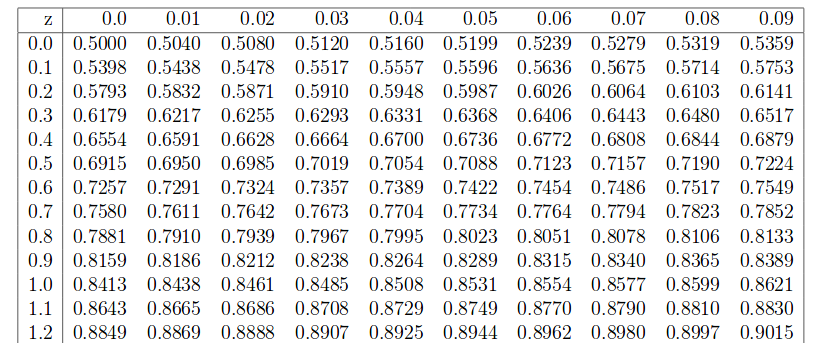
\includegraphics[scale=0.4]{normal1examen.jpg}
%\vspace{3cm}

\ifsol
$$\begin{aligned}
P(20< \overline{X}<25 /\overline{X}>20)&=\frac{P(20< \overline{X}<25\cap \overline{X}>20)}{1-P( \overline{X}\leq 20))}\\
&=\frac{F_Z\left(\frac{25-20}{\frac{50}{\sqrt{100}}}\right)-F_Z\left(\frac{20-20}{\frac{50}{\sqrt{100}}}\right)}{1-F_Z\left(\frac{20-20}{\frac{50}{\sqrt{100}}}\right)}=
\frac{F_Z(1)-F_Z(0)}{F_Z(0)}.
\end{aligned}$$
\fi


%\setcounter{problemes}{0}
\probl (\textbf{1 punto.}) Lanzamos un dado de 12 caras numeradas  con enteros del 1 al 12 sobre una mesa plana. Observamos el número superior del dado. Suponiendo equiprobabilidad de todas las caras calcular la probabilidad de que salga mayor que 8  si el resultado es par.

\ifsol
$$ P(X>8/X\in\{2,4,6,8,10,12\})=\frac{P(X\in\{10,12\})}{P(X\in\{2,4,6,8,10,12\})}=\frac{2/12}{6/12}=\frac{1}{3}.$$
\fi

\vspace{3cm}

\probl Lanzamos una moneda con probabilidad de cara $p=\frac{1}{2}$ hasta que sale cara dos veces  o bien la hemos lanzamos 5 veces, lo primero que ocurra.

Denotemos por $X$ la variable aleatoria que determina el número de tiradas de la moneda.

Se pide: 

\punt Describid adecuadamente el espacio muestral de la variable $X$. (\textbf{0.5 punto.})

\punt Calcular  su función de densidad.(\textbf{1 punto.})

\punt Calcular $E(X)$.(\textbf{1 punto.})

\ifsol

$C$= cara $+$=cruz 
$$\begin{aligned}\Omega=\{&CC,C+C,+CC,++CC,+C+C,C++C,+++CC,++C+C,+C++C,C+++C,\\ & +++++,C++++,+C+++,++C++,+++C+,++++C\}\end{aligned}.$$
$X=$ número de tiradas $D_X=\{2,3,4,5\}.$


$P(X=2)=\left(\frac{1}{2}\right)^2, P(X=3)=2\cdot\left(\frac{1}{2}\right)^3,P(X=4)=3\cdot\left(\frac{1}{2}\right)^4,P(X=5)=10\cdot \left(\frac{1}{2}\right)^5.$

$P(X=x)= (x-1)\cdot \left(\frac{1}{2}\right)^x$ si $x=2,3,4$, $P(X=5)=\frac{10}{32}$ y cero en el resto de casos.

$E(X)=2\cdot\frac{1}{4}+3\cdot \frac{1}{4}+ 4\cdot \frac{3}{16}+5\cdot \frac{10}{32}=\frac{57}{16}.$
\fi 

\probl Sea $X$  una variable  con distribución uniforme en el intervalo $(1,10)$ con  $a>1$. Consideremos la variable $Y=\log_{10}(X)$. Se pide

\punt Calcular la función de distribución  de $Y$ (\textbf{1 punto.}) 

\punt Calcular la función de densidad de $Y$. (\textbf{0.5 puntos.})

\punt Calcular el cuantil 0.95 de $Y$. (\textbf{0.5 puntos.})

\ifsol

Recordemos que 
$$
F_X(x)=\left\{
\begin{array}{ll} 
0 & \mbox{si} x\leq 0\\
\frac{x-1}{9} & \mbox{si} 0< x < 10\\
1 & \mbox{si} x\geq 10
\end{array}\right.
$$

La variable $Y$ tendrá por dominio $D_Y=(0,1)$.

Sea $y\in(0,1)$ entonces $F_Y(y)=P(Y\leq y)=P(\log(X)\leq y)=P(X\leq 10^y)=\frac{10^y-1}{9}$ ya que  como $0<y<1$ entonces
$0< 10^y < 10$.  Así que la función de distribución es 

$$
F_Y(y)=\left\{\begin{array}{ll} 
0 & \mbox{si} x\leq 0\\
\frac{10^y-1}{9} & \mbox{si} 0< y < 1\\
1 & \mbox{si} y\geq 1\\
\end{array}\right.
$$
 su densidad es 

% $$
% f_y(y)=F'_Y(y)=
% =\left\{\begin{array}{ll} 
% \frac{10^y\cdot log_e(10)}{9} & \mbox{si} 0< y < 1\\
% 0 & \mbox{en cualquier otro caso}\\
% \end{array}\right}
% $$



$E(Y)=E(\log_{10}(X))=\int_{0}^{1} \log_{10}(X)\cdot 1 dx=$
\fi

\probl  \textbf{(0.5 puntos)} 
Sea $X$ una v.a. discreta de dominio $D_X=\{-2,-1,0,1,2\}$. Sabemos que $P(X=x)=p$ para $x\in D_X$.
Calculad $Var(X)$.

\ifsol
\textbf{Solución:}

\sl

$\frac{2}{5}.$
\else
%\vspace*{1cm}

\fi


\probl  \textbf{(0.5 puntos)} 
Sea $Z$ una variable aleatoria normal estándar.  Tenemos que \texttt{pnorm(-0.2)}=0.4207.
Calculad $P(|Z|\geq 0.2)$.

\ifsol
\textbf{Solución:}

\sl

0.8415.
\else
%\vspace*{1cm}

\fi




\probl \textbf{(2 puntos)}  Consideremos la v.a. $X$ con función densidad


$$f(x)=\left\{
\begin{array}{cl}
 \displaystyle 0.5& \mbox{si } 0< x <1 \\
\displaystyle\frac{x-1}{2} & \mbox{si } 1\leq x < a \\
 \displaystyle 0 & \mbox{ en cualquier otro caso } \\
\end{array}\right..
$$

\begin{enumerate}[a)]
\item Calculad el valor de $a$ para que $f$ sea función de densidad.
\item Para el anterior valor de $a$ calculad la función de distribución de $X$.
\item Para el anterior valor de $a$ calculad $E(X)$.
%\item Para el anterior valor de $a$ calculad $Var(X)$.
\end{enumerate}



\end{document}



